%        File: policy.tex
%     Created: Sun Mar 31 03:00 PM 2013 C
% Last Change: Sun Mar 31 03:00 PM 2013 C
%


%\documentclass[11pt,handout]{beamer}
\documentclass[9pt]{beamer}
\usetheme[white]{Wisconsin}
%\title[short title]{long title}
\title[U.S. Nuclear Waste Policy]{U.S. Nuclear Waste Policy, A History}
%\subtitle[short subtitle]{long subtitle}
\subtitle[NE571]{NE571}
%\author[short name]{long name}
\author[Kathryn D. Huff]{Kathryn D. Huff}
%\date[short date]{long date}
\date[4.1.2013]{April 1, 2013}
%\institution[short name]{long name}
\institute[UW-Madison]{University of Wisconsin-Madison}

%\usepackage{bbding}
\usepackage{amsfonts}
\usepackage{amsmath}
\usepackage{graphicx}
\usepackage{subfigure}
\usepackage{booktabs} % nice rules for tables
\usepackage{microtype} % if using PDF
\usepackage{bigints}
\newcommand{\units}[1] {\:\text{#1}}%
\newcommand{\SN}{S$_N$}%{S$_\text{N}$}%{$S_N$}%
\DeclareMathOperator{\erf}{erf}

%page numbers
\setbeamertemplate{footline}[page number]
%Those icons in the references are terrible looking
\setbeamertemplate{bibliography item}[text]
\begin{document}
%%%%%%%%%%%%%%%%%%%%%%%%%%%%%%%%%%%%%%%%%%%%%%%%%%%%%%%%%%%%%
%% From uw-beamer Here's a handy bit of code to place at 
%% the beginning of your presentation (after \begin{document}):
\newcommand*{\alphabet}{ABCDEFGHIJKLMNOPQRSTUVWXYZabcdefghijklmnopqrstuvwxyz}
\newlength{\highlightheight}
\newlength{\highlightdepth}
\newlength{\highlightmargin}
\setlength{\highlightmargin}{2pt}
\settoheight{\highlightheight}{\alphabet}
\settodepth{\highlightdepth}{\alphabet}
\addtolength{\highlightheight}{\highlightmargin}
\addtolength{\highlightdepth}{\highlightmargin}
\addtolength{\highlightheight}{\highlightdepth}
\newcommand*{\Highlight}{\rlap{\textcolor{HighlightBackground}{\rule[-\highlightdepth]{\linewidth}{\highlightheight}}}}
%%%%%%%%%%%%%%%%%%%%%%%%%%%%%%%%%%%%%%%%%%%%%%%%%%%%%%%%%%%%%
%%--------------------------------%%
\frame{
  \titlepage
}

\section{Overview}
%%--------------------------------%%
\begin{frame}
  \frametitle{Outline}
  \tableofcontents[currentsection]
\end{frame}

\subsection{Waste Challenges}

%%--------------------------------%%
\begin{frame}[ctb!]
  \frametitle{Spent Nuclear Fuel}
  \begin{figure}[htb!]
  \begin{center}
    \includegraphics[height=0.7\textheight]{fuel_assembly.eps}
  \end{center}
  \caption{Spent nuclear fuel from conventional power reactors is in the form of 
    uranium oxide fuel rods \cite{nrc_nuclear-fuel.jpg_????}.}
  \label{fig:snf}
\end{figure}

\end{frame}

%%--------------------------------%%
\begin{frame}[ctb!]
  \frametitle{Other High Level Wastes}
  \begin{itemize}
    \item Navy Spent Fuel
    \item Defense Wastes
    \item Reprocessing Wastes
  \end{itemize}
\end{frame}

%%--------------------------------%%
\begin{frame}[ctb!]
  \frametitle{Current Locations of SNF and HLW}
  
\begin{figure}[htb!]
  \begin{center}
    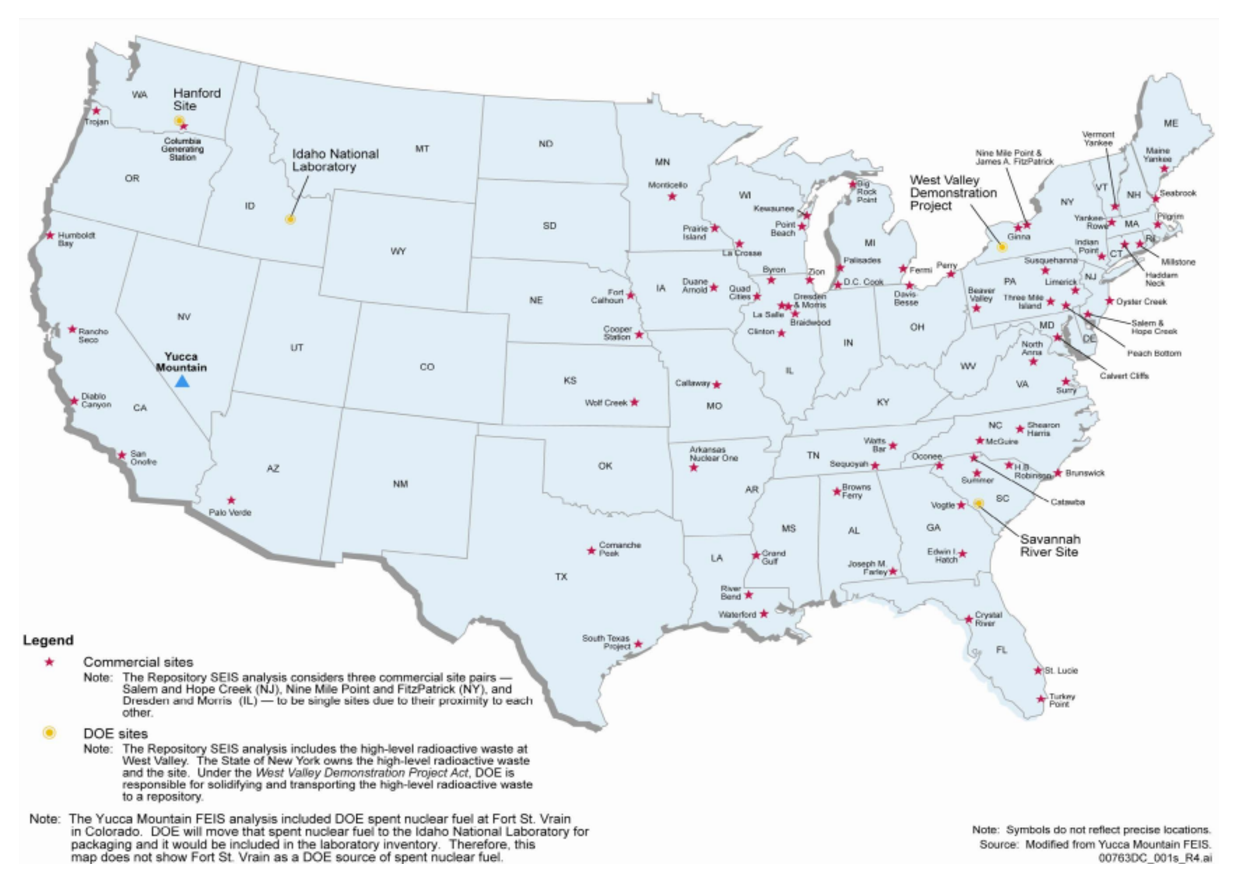
\includegraphics[width=\linewidth]{locations.eps}
  \end{center}
  \caption{The locations of the used nuclear fuel and high level waste in the 
  united states cover over a hundred locations and nearly 40 states 
  \cite{doe_final_2008}}
  \label{fig:locations}
\end{figure}

\end{frame}

%%--------------------------------%%
\begin{frame}[ctb!]
  \frametitle{Current Storage of SNF and HLW}
  

  \begin{figure}[htbp!]
    \begin{center}
    \begin{minipage}[t]{0.45\textwidth}
      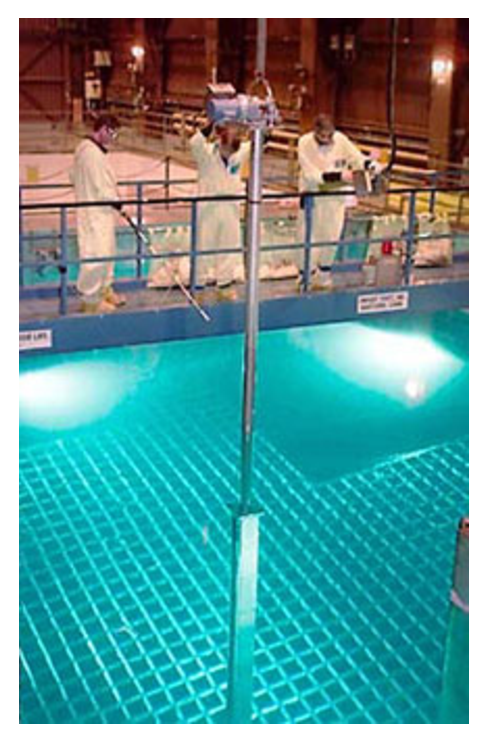
\includegraphics[height=0.4\textheight]{pool.eps}
      \caption{Spent fuel pools are at reactor sites and elsewhere 
        \cite{doe_spent_????}.}
        \label{fig:pool}
    \end{minipage}
    \hspace{0.01\textwidth}
    \begin{minipage}[t]{0.45\textwidth}
      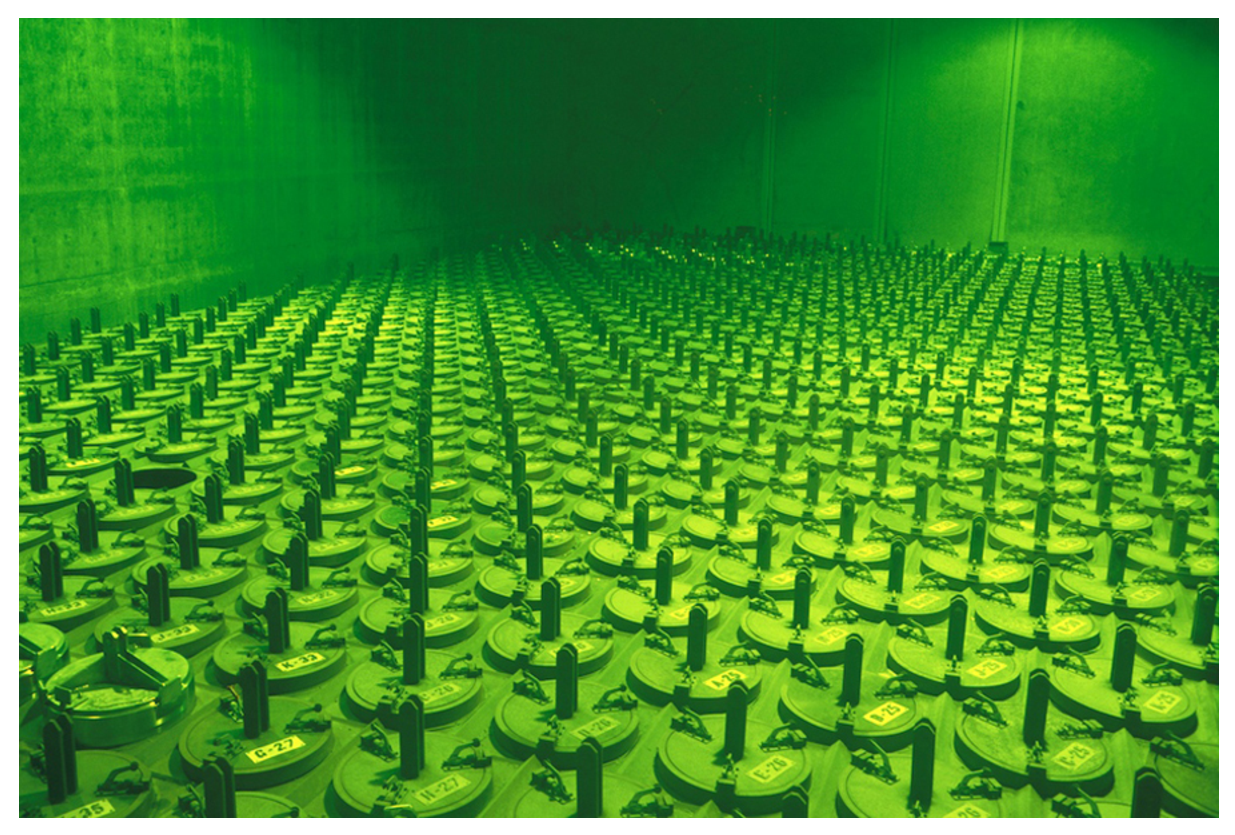
\includegraphics[height=0.4\textheight]{logs.eps}
        \caption{Vitrified glass logs at reprocessing facilities and elsewhere 
          \cite{essick_photographing_2012}.}
        \label{fig:logs}
    \end{minipage}
    \end{center}
  \end{figure}

\end{frame}

%%--------------------------------%%
\begin{frame}[ctb!]
  \frametitle{Current Storage of SNF and HLW}
  

  \begin{figure}[htbp!]
    \begin{center}
    \begin{minipage}[t]{0.45\textwidth}
      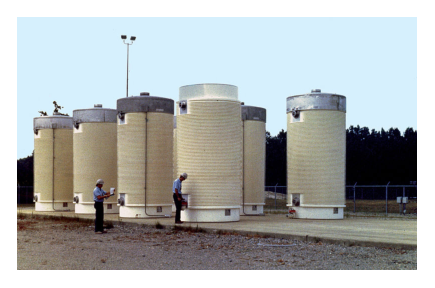
\includegraphics[height=0.4\textheight]{casks.eps}
      \caption{Dry casks at reactor sites and elsewhere \cite{nrc_dry_2008}}
        \label{fig:casks}
    \end{minipage}
    \hspace{0.01\textwidth}
    \begin{minipage}[t]{0.45\textwidth}
      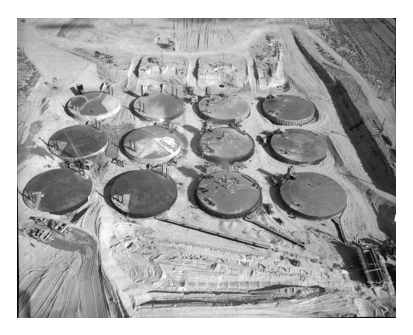
\includegraphics[height=0.4\textheight]{tanks.eps}
        \caption{Liquid waste in steel or carbon steel tanks at Hanford and 
          elsewhere\cite{doe_underground_????}.}
        \label{fig:tanks}
    \end{minipage}
    \end{center}
  \end{figure}

\end{frame}

%%--------------------------------%%
\begin{frame}[ctb!]
  \frametitle{How Much?}
  \begin{figure}[htbp!]
  \begin{center}
    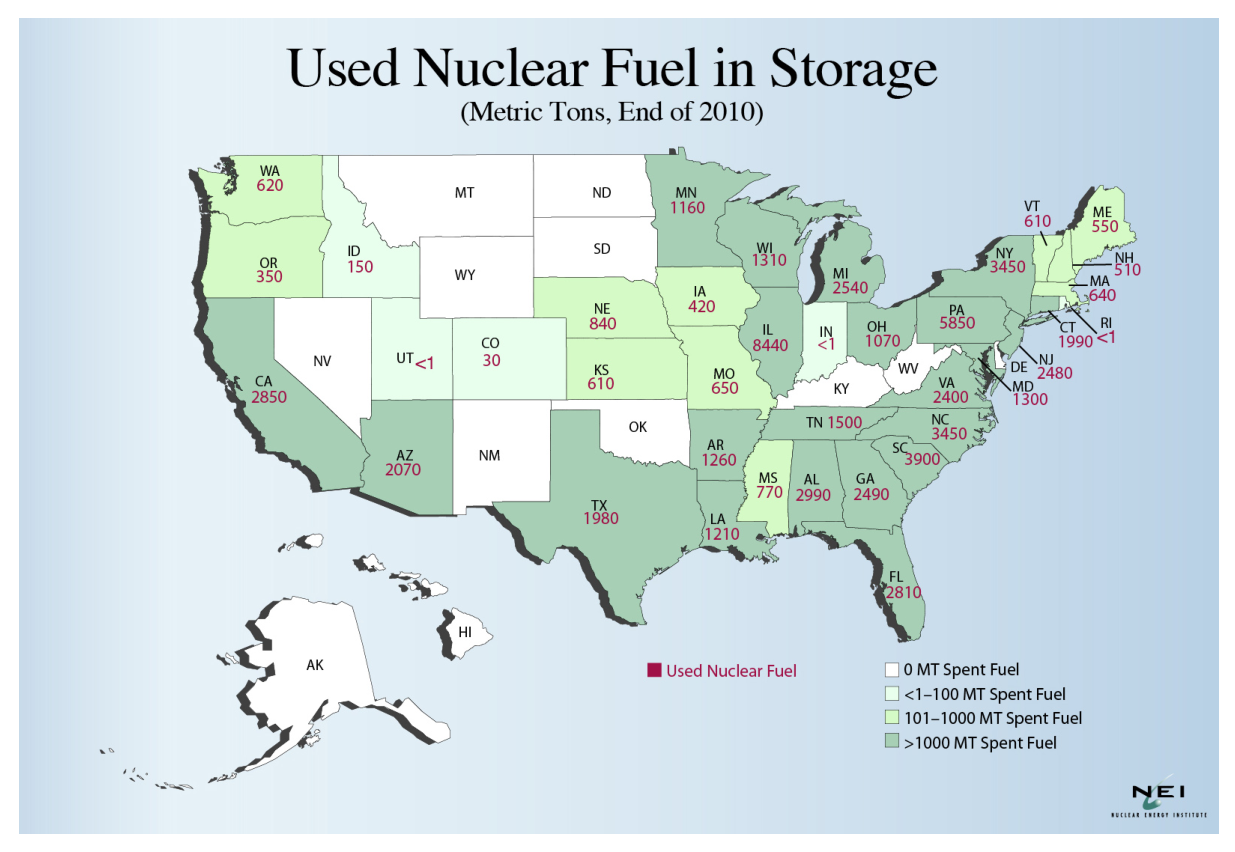
\includegraphics[height=0.7\textheight]{metric_tons.eps}
  \end{center}
  \caption{The amount of nuclear spent fuel and high level waste now exceeds the 
    proposed legislative capacity of Yucca Mountain \cite{peters_whats_2013}}
  \label{fig:metric_tons}
\end{figure}

\end{frame}


\subsection{Management Options}

%%--------------------------------%%
\begin{frame}[ctb!]
    \frametitle{Array of Possible Options}
    \begin{figure}[htbp!]
  \begin{center}
    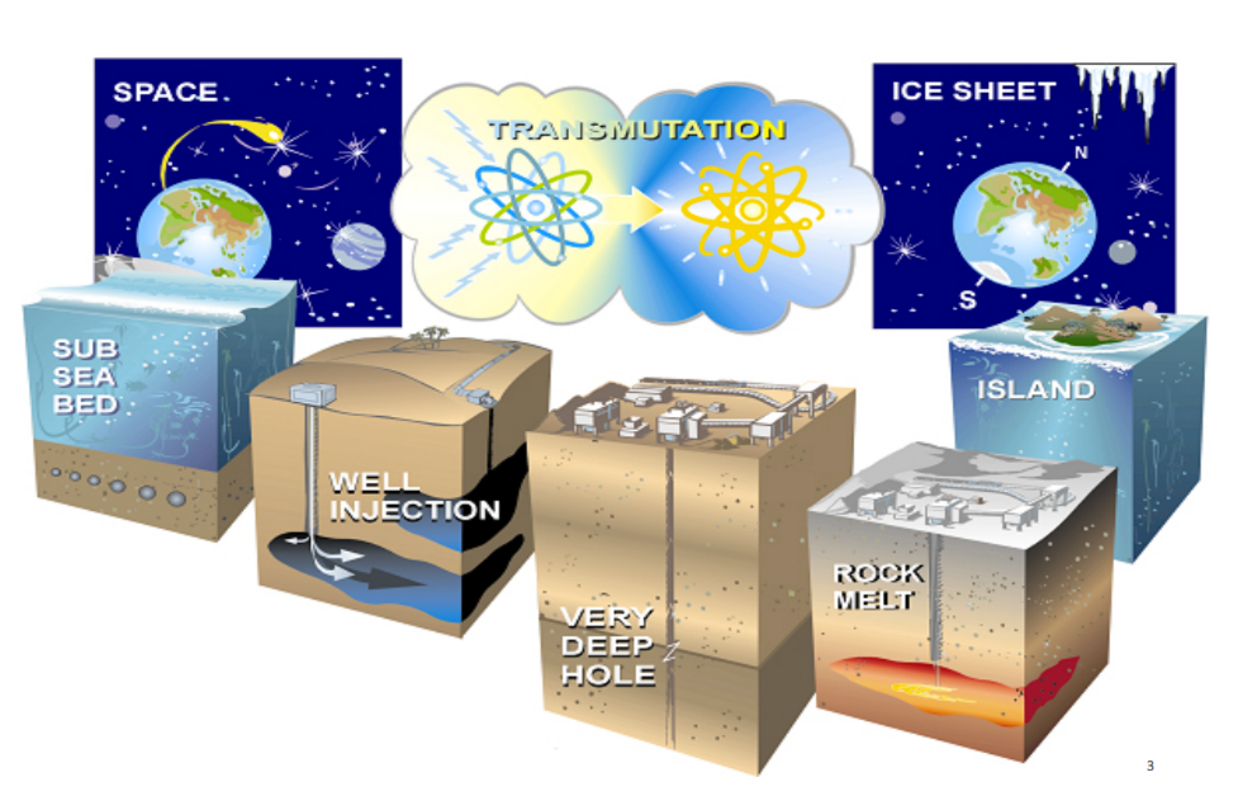
\includegraphics{alternative_options.eps}
  \end{center}
  \caption{An array of options have been considered in the past 
    \cite{peters_what_2013}.}
  \label{fig:alternative_options}
\end{figure}

  \end{frame}

%%--------------------------------%%
\begin{frame}[ctb!]
    \frametitle{Geologic Disposal}
    \begin{figure}[htbp!]
  \begin{center}
    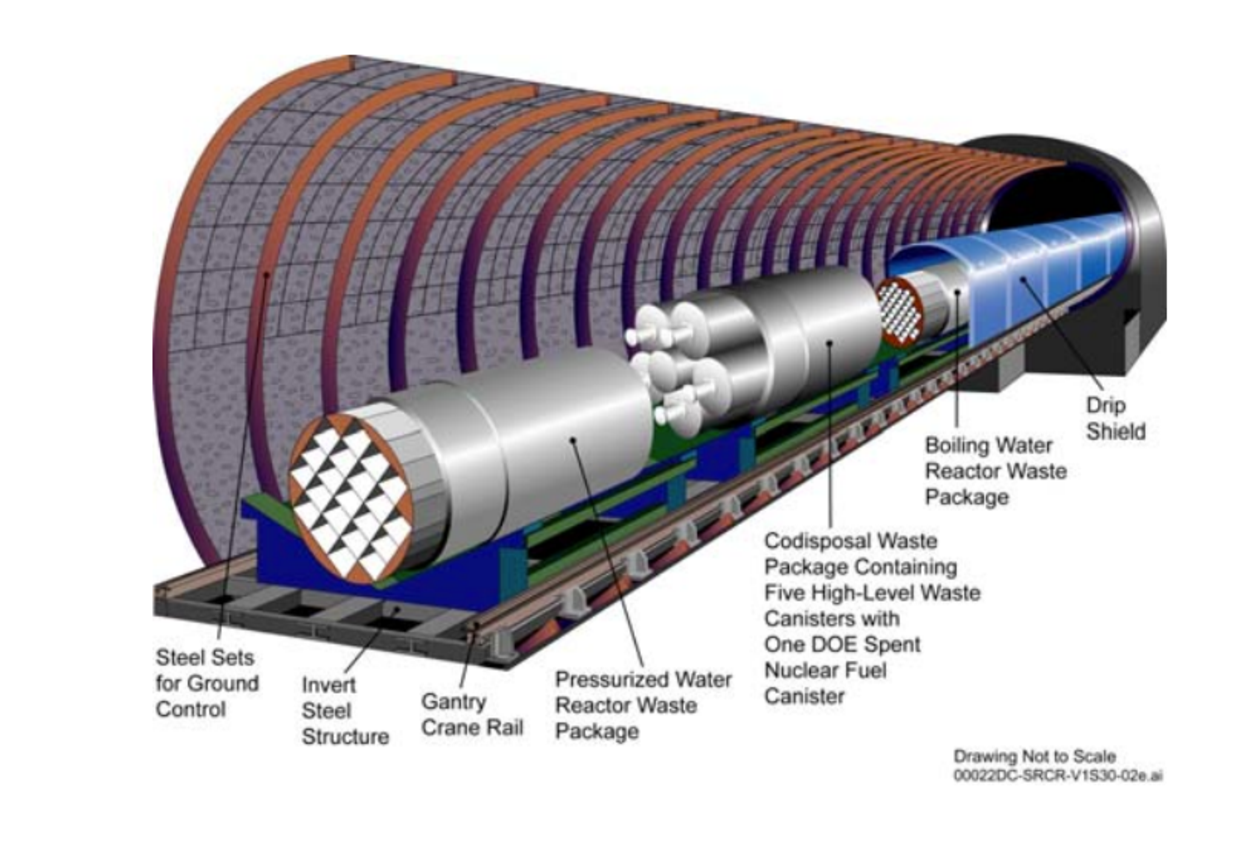
\includegraphics[height=0.7\textwidth]{yucca_tunnel.eps}
  \end{center}
  \caption{The current U.S. geologic disposal concept \cite{peters_whats_2013}.}
  \label{fig:yucca_tunnel}
\end{figure}

  \end{frame} 



\section{History}
\subsection{Pre-NWPA}

%%--------------------------------%%
\begin{frame}[ctb!]
  \frametitle{History}
  \begin{figure}[htbp!]
  \begin{center}
    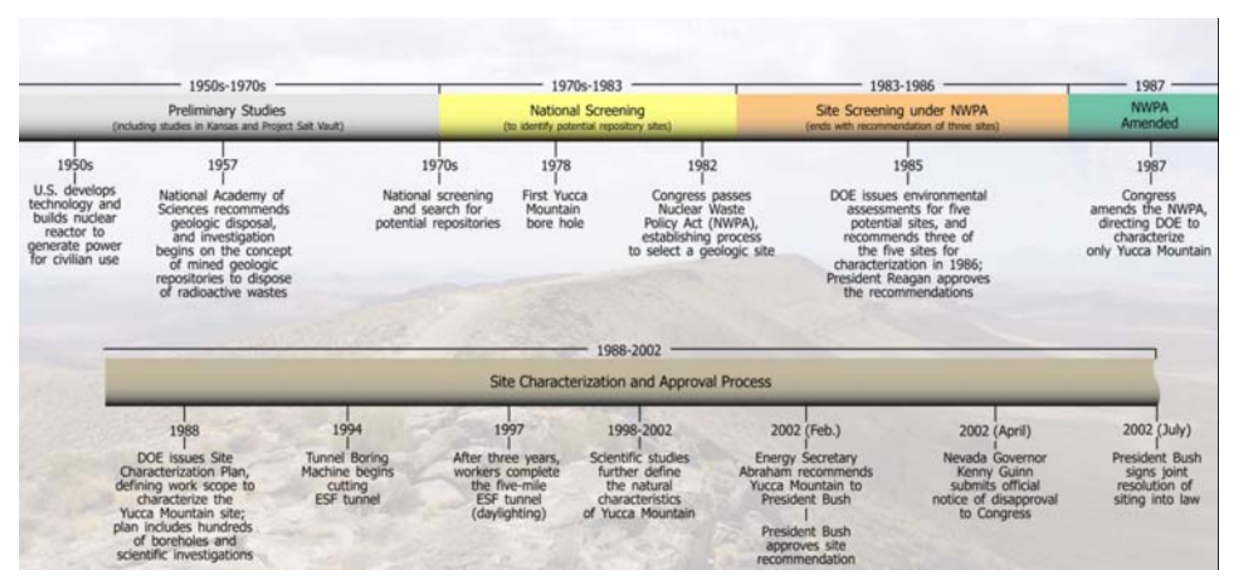
\includegraphics[width=0.8\textwidth]{timeline.eps}
  \end{center}
  \caption{The full history of domestic nuclear waste policy, in eras 
    \cite{peters_whats_2013}.}
  \label{fig:timeline}
\end{figure}

\end{frame}
%%--------------------------------%%
\begin{frame}[ctb!]
  \frametitle{1950-1970 Preliminary Studies}
  \begin{itemize}
    \item 1940s - first defense waste produced
    \item 1950s - first power reactors
    \item 1957 - National Academy of Sciences recommends geological disposal.
  \end{itemize}
\end{frame}

%%--------------------------------%%
\begin{frame}[ctb!]
  \frametitle{1970 - 1983 National Site Screening}
  \begin{itemize}
    \item 1978 - first Yucca Mountain Borehole
    \item 1982 - Nuclear Waste Policy Act
  \end{itemize}
\end{frame}


\subsection{NWPA}

%%--------------------------------%%
\begin{frame}[ctb!]
  \frametitle{1983 Nuclear Waste Policy Act}
  Passed through congress in 1982, it was signed into law in January, 1983 by 
  President Jimmy Carter?

  \begin{quotation}
    This legislation defined the Federal Government’s responsibility to provide 
    permanent disposal in a deep geologic repository for spent fuel and high-level 
    radioactive waste from commercial and defense activities. Under amended 
    provisions (1987)  of this Act, the Department of Energy (DOE) has the 
    responsibility to locate, build, and operate a repository for such wastes. 
    \cite{nrc_backgrounder_2011}
  \end{quotation}

\end{frame}

%%--------------------------------%%
\begin{frame}[ctb!]
  \frametitle{Nuclear Waste Fund}
  The NWPA established a nuclear waste fund, to be paid into by the commercial 
  entities producing nuclear waste domestically.
  \begin{quotation}
    In return for 1 mill per kWh, the utilities would gain the assurance that 
    the United States would manage the disposal of that waste.
  \end{quotation}

\end{frame}

%%--------------------------------%%
\begin{frame}[ctb!]
  \frametitle{Nuclear Waste Fund}
  Though some of the Nuclear Waste Fund has been spent on the Yucca Mountain 
  Project, it currently has an unspent balance of \$25 billion. 

  It receives nearly \$750 million each year from the commerical entities that 
  pay into it.
\end{frame}


%%--------------------------------%%
\begin{frame}[ctb!]
  \frametitle{Site Review}
  \begin{figure}[htbp!]
  \begin{center}
    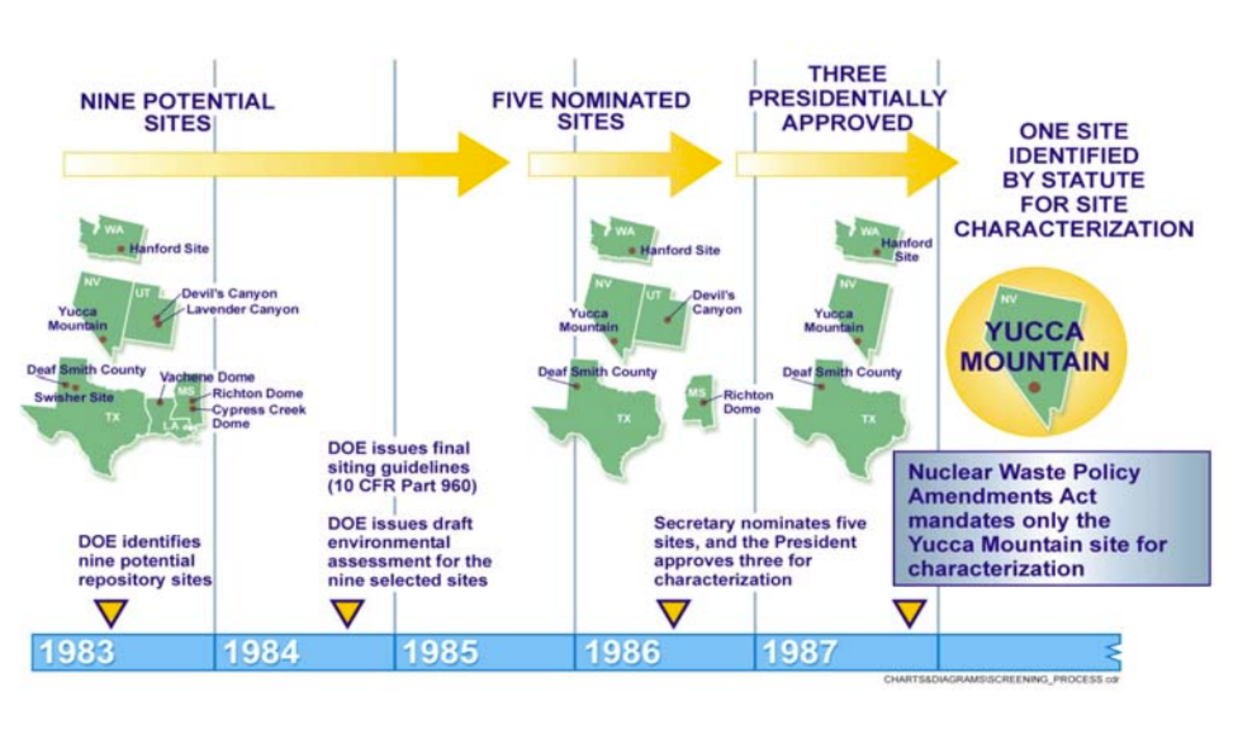
\includegraphics{nine_sites_to_one.eps}
  \end{center}
  \caption{The siting process began at nine sites and downselected to one 
    \cite{peters_what_2013}.}
  \label{fig:nine_sites_to_one}
\end{figure}

\end{frame}

%%--------------------------------%%
\begin{frame}[ctb!]
  \frametitle{Selection of Yucca Mountain}

  The Yucca Mountain Site was selected and accepted by the office of President 
  Ronal Reagan in 1987. Further spent fuel disposal R\&D would work toward a 
  lisence applicaton for the Yucca Mountain Site. 
  \begin{figure}[htbp!]
  \begin{center}
    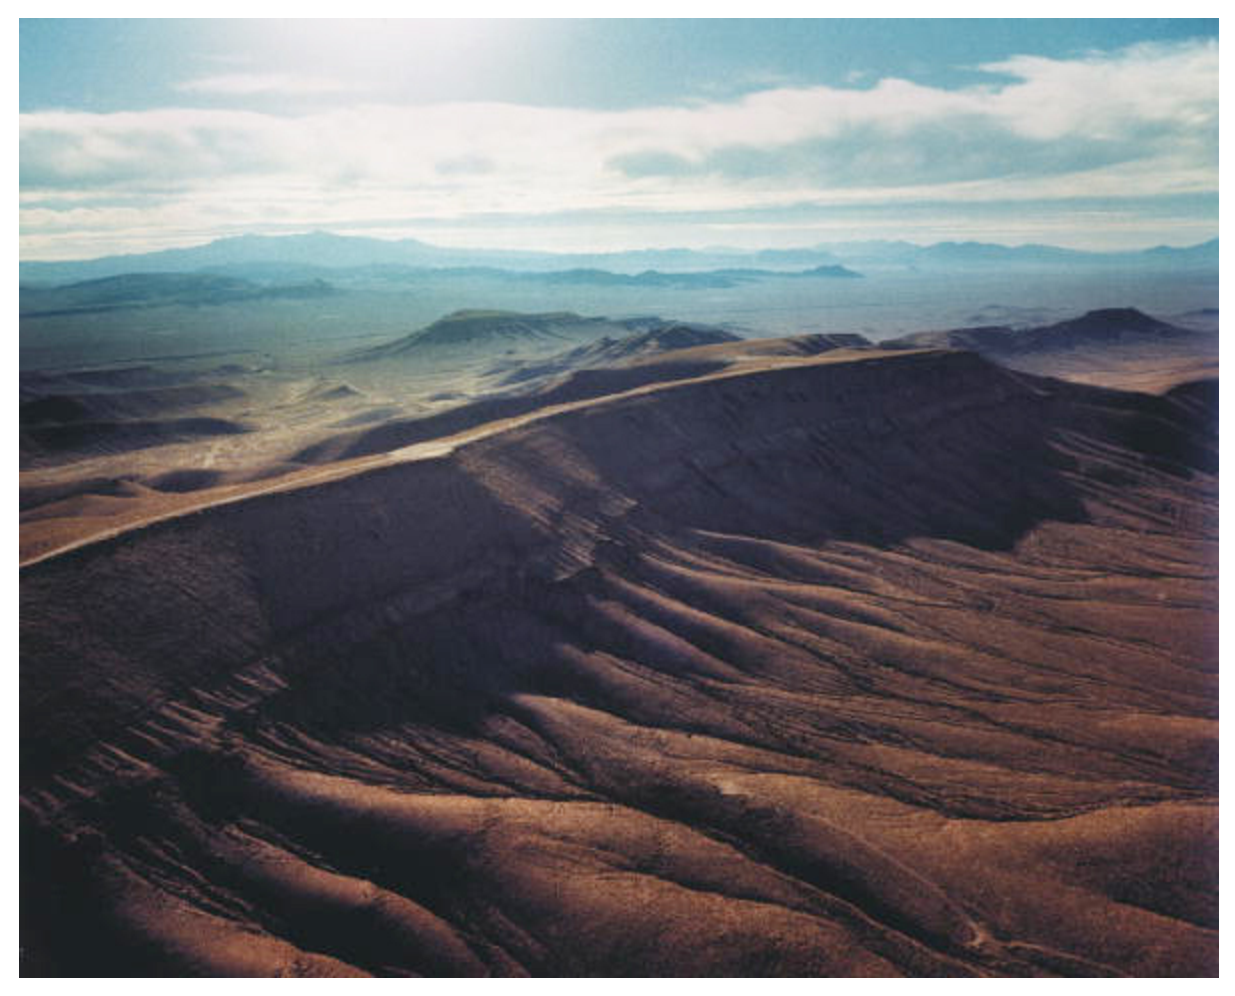
\includegraphics{yucca_site.eps}
  \end{center}
  \caption{Yucca Mountain in southern Nevada \cite{wherever_you_got_this}.}
  \label{fig:yucca_site}
\end{figure}

\end{frame}

\subsection{Yucca Mountain Project}

%%--------------------------------%%
\begin{frame}[ctb!]
    \frametitle{1988 Viability Assessment}
    The Yucca Mountain site was deemed a viable site for further 
    characterization and the pursuit of a license application began. 

  \end{frame}

%%--------------------------------%%
\begin{frame}[ctb!]
    \frametitle{1988-2002 Site Characterization}
    The Yucca Mountain site was characterized 
    \begin{itemize}
      \item a huge team of people 
      \item over the span of 15 years
      \item under the regulation and direction of many government agencies.
    \end{itemize}
  \end{frame}

%%--------------------------------%%
\begin{frame}[ctb!]
\frametitle{Nuclear Waste Fund Litigation}
    \begin{itemize}
    \item 1983 - Nuclear utilities signed the Standard Contract agreeing to pay the nuclear waste fee.
    \item 1998 - The utilities sue the federal government over the delay in used fuel acceptance.
    \item 1998 - Courts ruled the DOE is partially liable. DOE settled. 
    \item ? - DOE developed an amended Standard Contract
  \end{itemize}
\end{frame}

%%--------------------------------%%
\begin{frame}[ctb!]
    \frametitle{2002 - Site Recommendation}
    The site was deemed appropriately characterized for recommendation in 2002.

    \vspace{3cm}
      \textbf{Secretary of Energy}$\longrightarrow$\textbf{President 
      Bush}$\longrightarrow$\textbf{Congress}
  \end{frame}

%%--------------------------------%%
\begin{frame}[ctb!]
    \frametitle{2008 - 2013 License Application and Withdrawal}
    \begin{itemize}
      \item The license application was \textbf{submitted} to the NRC in 2008.
      \item The NRC was expected to make a decision \textbf{within 4 years}.
      \item In \textbf{May 2009}, Secretary Steven Chu stated: ``Yucca Mountain as a 
        repository is off the table''.
      \item \textbf{July 2009}, the House of Representatives voted 388 to 30 to 
        not defund the Yucca Mountain repository in the FY2010 budget.
      \item On \textbf{March 3, 2010}, the DOE filed a motion with the NRC to 
        withdraw its license application. 
      \item YMP funding was terminated with the Defense and Full-Year Continuing 
        Appropriations Act, passed by Congress on \textbf{April 14, 2011}.
    \end{itemize}
  \end{frame}





\section{Outlook}
\subsection{BRC}

%%--------------------------------%%
\begin{frame}[ctb!]
    \frametitle{Blue Ribbon Commission Charter}
    The goals of the blue ribbon commission were:
    \begin{itemize}
      \item <++>
      \item <++>
      \item <++>
      \item <++>
      \item <++>
      \item <++>
      \item <++>
    \end{itemize}

  \end{frame}

%%--------------------------------%%
\begin{frame}[ctb!]
    \frametitle{Recommendations from the BRC}
    The BRC came out with a list of recommendations
    \begin{itemize}
      \item <++>
      \item <++>
      \item <++>
      \item <++>
      \item <++>
      \item <++>
      \item <++>
    \end{itemize}
  \end{frame}

%%--------------------------------%%
\begin{frame}[ctb!]
    \frametitle{DOE Response to the BRC}

    DOE began created four working groups. 
    \begin{itemize}
      \item Governance Framework and Funding
      \item System Design \& Architecture
      \item ConsentBased Siting
      \item Transportation Routing, Safety and Security
  \end{frame}

%%--------------------------------%%
\begin{frame}[ctb!]
    \frametitle{DOE Response to the BRC}

    In a brief statement \cite{doe_strategy_2011}, the DOE agreed in general 
    with the BRC that they should pursue:

    \begin{itemize}
      \item[$\checkmark$] An independent agency to oversee the Nuclear Waste 
        Fund ( though the TVA-style version is discouraged. )
      \item[$\checkmark$] <++> 
      \item[$\checkmark$] <++> 
      \item[$\checkmark$] <++> 
    \end{itemize}
  \end{frame}

%%--------------------------------%%
\begin{frame}[ctb!]
    \frametitle{Congressional Response to the BRC}
    Senator Jeff Bingaman, before leaving office, introduced a bill called the 
    Nuclear Waste Administration Act of 2011. It suggested an independent waste 
    fund management body of the administrative type. 

    The future of this bill is unknown. 
  \end{frame}


\subsection{Nuclear Waste Confidence Ruling}

%%--------------------------------%%
\begin{frame}
    \frametitle{Waste Confidence}
    To license a reactor or approve a reactor license extension, the NRC 
    requires a Waste Confidence clause. It is a section of the application that 
    assures the NRC that waste produced by the applying facility will be dealt 
    with. 

    Previous to the closing of the Yucca Mountain Project, all applicants for 
    reactor licenses and license extensinos were able to cite the nuclear waste 
    fund and the Yucca Mountain Project. 

    This is no longer the case. 
  \end{frame}

%%--------------------------------%%
\begin{frame}
    \frametitle{Waste Confidence Ruling}
    In 2012, the United States Court of Appeals for the District of Columbia Circuit declared that there is no waste confidence. 
    
    \begin{quotation} 
      ``The commission apparently has no long-term plan other than hoping for a
        geologic repository... Failing to establish a repository is a
        possibility thatcannot be ignored.'' \cite{sentelle_petitions_2012} 
    \end{quotation}
  \end{frame}


\subsection{Yucca Mountain License Application Proceedings}

%%--------------------------------%%
\begin{frame}[ctb!]
    \frametitle{Yucca Mountain License Application Litigation}
    ?

  \end{frame}




%%----------------------------------------%%
\begin{frame}[ctb!]
  \frametitle{Conclusion}
  Thanks!
  
  Feel free to direct questions to huff2@wisc.edu.
\end{frame}

%%--------------------------------%%
%%--------------------------------%%
\begin{frame}[allowframebreaks]
  \frametitle{References}
  \bibliographystyle{plain}
  {\footnotesize \bibliography{ne571} }

\end{frame}

%%--------------------------------%%




\end{document}





